\documentclass{article}
\usepackage[utf8]{inputenc}
\usepackage[english]{babel}
\usepackage{graphicx}
\usepackage{subfigure}
\usepackage{apacite}
\usepackage{amssymb}
\usepackage{amsmath}
\usepackage{epstopdf}
\usepackage[utf8]{inputenc}
\usepackage{tikz-cd,amsmath}
\usepackage{amsfonts}
\usepackage{amsthm}
\usepackage{ulem}
\usepackage{fancyhdr}
\usepackage{graphicx}
\usepackage{tikz}
\usepackage{tikz-3dplot}
\graphicspath{ {./images/} }
\usepackage{array}
\usepackage{mathrsfs}
\usepackage{tikz,tikz-cd}
\usepackage{float}
\usepackage{amsmath,esint}

\usepackage{hyperref}
\hypersetup{
    colorlinks=true,
    linkcolor=blue,
    filecolor=magenta,      
    urlcolor=cyan,
}

\usepackage{geometry}
 \geometry{
 a4paper,
 %total={170mm,257mm},
 left=25mm,
 right=25mm,
 top=20mm,
 }

\theoremstyle{definition}
\newtheorem{problem}{Problem}
\theoremstyle{definition}
\newtheorem{definition}{Definition}
\theoremstyle{definition}  
\newtheorem{lemma}{Lemma}
\theoremstyle{definition}
\newtheorem{proposition}{Proposition}
\theoremstyle{definition}
\newtheorem{remark}{Remark}
\theoremstyle{definition}
\newtheorem{example}{Example}
\theoremstyle{definition}
\newtheorem{question}{Question}
\theoremstyle{definition}
\newtheorem{Question}{Follow-up Question}
\theoremstyle{definition}
\newtheorem{exercise}{Exercise}

\newtheorem{theorem}{Theorem}[section]
\newtheorem{corollary}{Corollary}[theorem]

\newcommand{\RR}{\mathbb{R}}
\newcommand{\ZZ}{\mathbb{Z}}
\newcommand{\QQ}{\mathbb{Q}}
\newcommand{\CC}{\mathbb{C}}

\title{Calculus}
\author{Kevin }
\date{April 2021}

\begin{document}

\maketitle
\tableofcontents
%\pagebreak
\section{Two Standard Limits}
The following two standard limits are important for differentiating trigonometric functions from the first principle, i.e., by definition.
\begin{align}
    \lim_{\theta\to0}\dfrac{\sin(\theta)}{\theta}=1\\
    \lim_{\theta\to0}\dfrac{\cos(\theta)-1}{\theta}=0
\end{align}
The proof is essentially about establishing an upper and lower bound for these two functions.
\begin{proof}
We prove the first one by squeeze lemma. We know that the following inequality is true on a sufficient small neighborhood $(-\epsilon,\epsilon)$ around the origin.
\[|\sin(\theta)|\le|\theta|\le|\tan(\theta)|\]
This is equivalent to
\[\left|\dfrac{\sin(\theta)}{\theta}\right|\le 1\le \left|\dfrac{\sin(\theta)}{\theta\cos(\theta)}\right|\]

Rearranging the second inequality above gives
\[|\cos(\theta)|\le\left|\dfrac{\sin(\theta)}{\theta}\right|\]
Hence,
\begin{equation}
    |\cos(\theta)|\le \left|\dfrac{\sin(\theta)}{\theta}\right|\le1
\end{equation}
By squeeze lemma,
\begin{equation}
    \lim_{\theta\to0}|\cos\theta|\le\lim_{\theta\to0}\left|\dfrac{\sin(\theta)}{\theta}\right|\le \lim_{\theta\to0}1
\end{equation}
which implies that $\lim_{\theta\to0}\frac{\sin(\theta)}{\theta}=1$. However, to assert that the limit of this function exist, one needs to appeal to some $\epsilon$-$\delta$ argument to prove that the limits from both sides exist and agree.

There is a proof of the second limit in Haese (textbook). I'll present a different proof that still uses squeeze lemma. Note that \[
\left|\dfrac{1-\cos(\theta)}{\theta}\right|\ge 0
\]
holds trivially. This will be our lower bound.
Now, consider the unit circle $S^1=\{(x,y)\in\mathbb{R}^2\mid x^2+y^2=1\}$ and the following diagram (using Geogebra).
\begin{figure}[H]
    \centering
    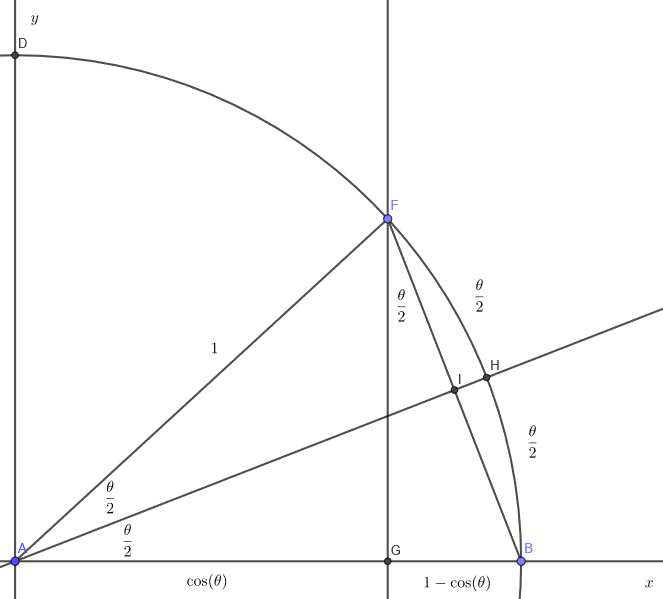
\includegraphics[scale=0.6]{Pictures/Trig_limit.PNG}
    \caption{Geometric proof}
    \label{fig:my_label}
\end{figure}
It is easy to prove that $\triangle AIB\sim \triangle FGB$. $\because$ $AH$ divides the angle $\theta$ into two equivalent parts, $\therefore$ $\angle GFB=\frac{\theta}{2}$. By the definition of $\sin(\theta)$, we have 
\[
\sin\left(\dfrac{\theta}{2}\right)=\dfrac{BG}{FB}=\dfrac{1-\cos(\theta)}{FB}\ge \dfrac{1-\cos(\theta)}{\theta}
\]
Hence,
\begin{equation}
    0\le\left|\dfrac{1-\cos(\theta)}{\theta}\right|\le \sin\left(\dfrac{\theta}{2}\right)
\end{equation}
By squeeze lemma, 
\begin{equation}
    \lim_{\theta\to0}0\le\lim_{\theta\to0}\left|\dfrac{1-\cos(\theta)}{\theta}\right|\le \lim_{\theta\to0}\sin\left(\dfrac{\theta}{2}\right)
\end{equation}
which implies that $\lim_{\theta\to0}\frac{\cos(\theta)-1}{\theta}=-\lim_{\theta\to0}\frac{1-\cos(\theta)}{\theta}=0$.
\end{proof}

\section{The Derivatives of Trigonometric Functions (First Principle)}
\subsection{Sine and Cosecant}
Let's start......
\begin{align*}
    \dfrac{d}{dx}\sin(x)=\lim_{h\to0}\dfrac{\sin(x+h)-\sin(x)}{h}\\
    =\lim_{h\to0}\dfrac{\sin(x)\cos(h)+\sin(h)\cos(x)-\sin(x)}{h}\\
    =\lim_{h\to0}\dfrac{\sin(x)(\cos(h)-1)+\cos(x)\sin(h)}{h}\\
    =\sin(x)\lim_{h\to0}\dfrac{\cos(h)-1}{h}+\cos(x)\lim_{h\to0}\dfrac{\sin(h)}{h}\\
    =\cos(x)
\end{align*}

Two methods for driving the derivative of Cosecant.\\
\textbf{Method 1:}\\
$\csc$ is the reciprocal of $\sin$, so let $u=\sin(x)$, then
\begin{align*}
    \dfrac{d}{dx}\csc(x)=\dfrac{d}{du}\dfrac{1}{u}\dfrac{d}{dx}\sin(x)=-\dfrac{1}{u^2}\cos(x)=-\dfrac{\cos(x)}{\sin^2(x)}\\
    =-\csc(x)\cot(x)
\end{align*}

\textbf{Method 2 (First Principle):}\\
Start:
\begin{align*}
    \dfrac{d}{dx}\csc(x)=\lim_{h\to0}\left(\dfrac{1}{h}\left(\frac{1}{\sin(x+h)}-\frac{1}{\sin(x)}\right)\right)\\
    =\lim_{h\to0}\left(\dfrac{1}{h}\dfrac{\sin(x)-\sin(x+h)}{\sin(x+h)\sin(x)}\right)\\
    =\lim_{h\to0}\dfrac{2\sin((x-x-h)/2)\cos((2x+h)/2)}{h\sin(x+h)\sin(x)}\\
    =\lim_{h\to0}\dfrac{\sin((x-x-h)/2)\cos((2x+h)/2)}{\frac{h}{2}\sin(x+h)\sin(x)}\\
    =\lim_{h\to0}\dfrac{\sin(-h/2)}{h/2}\lim_{h\to0}\dfrac{\cos(x+h/2)}{\sin(x+h)\sin(x)}\\
    =-\dfrac{\cos(x)}{\sin^2(x)}\\
    =-\csc(x)\cot(x)
\end{align*}
\subsection{Cosine and Secant}
Can you complete these two similarly? (DO DO IT)

The details will not be as clear as the preceding subsection because I'm lazy, and I don't want to repeat similar argument.
\begin{align*}
    \dfrac{d}{dx}\cos(x)=\lim_{h\to0}\dfrac{\cos(x+h)-\cos(x)}{h}\\
    =\lim_{h\to0}\dfrac{\cos(x)\cos(h)-\sin(x)\sin(h)-\cos(x)}{h}\\
    =\cos(x)\lim_{h\to0}\dfrac{\cos(h)-1}{h}-\sin(x)\lim_{h\to0}\dfrac{\sin(h)}{h}\\
    =-\sin(x)
\end{align*}

Now we turn to $\sec(x)$. I'll skip the first method because it's similar to Method 1 of differentiating $\csc(x)$.
\begin{align*}
    \dfrac{d}{dx}\sec(x)=\lim_{h\to0}\dfrac{\cos(x)-\cos(x+h)}{h\cos(x+h)\cos(x)}\\
    =\lim_{h\to0}\dfrac{2\sin((2x+h)/2)\sin((x+h-x)/2)}{h\cos(x+h)\cos(x)}\\
    =\lim_{h\to0}\dfrac{\sin(x+h/2)}{\cos(x+h)\cos(x)}\lim_{h\to0}\dfrac{\sin(h/2)}{h/2}\\
    =\sec(x)\tan(x)
\end{align*}

\subsection{Tangent and Cotangent}
Use quotient rule to derive the derivative for these two if you are allowed to use it. Otherwise, use the following derivation.
\begin{align*}
    \dfrac{d}{dx}\tan(x)=\lim_{h\to0}\left(\dfrac{1}{h}\left(\dfrac{\sin(x+h)}{\cos(x+h)}-\dfrac{\sin(x)}{\cos(x)}\right)\right)\\
    =\lim_{h\to0}\dfrac{\sin(x+h)\cos(x)-\sin(x)\cos(x+h)}{h\cos(x+h)\cos(x)}\\
    =\lim_{h\to0}\dfrac{\sin(x+h-x)}{h\cos(x+h)\cos(x)}\\
    =\lim_{h\to0}\dfrac{\sin(h)}{h}\lim_{h\to0}\dfrac{1}{\cos(x+h)\cos(x)}
    =\dfrac{1}{\cos^2(x)}\\
    =\sec^2(x)
\end{align*}

For Cotangent,
\begin{align*}
    \dfrac{d}{dx}\cot(x)=\lim_{h\to0}\left(\dfrac{1}{h}\left(\dfrac{\cos(x+h)}{\sin(x+h)}-\dfrac{\cos(x)}{\sin(x)}\right)\right)\\
    =\lim_{h\to0}\dfrac{\cos(x+h)\sin(x)-\cos(x)\sin(x+h)}{h\sin(x+h)\sin(x)}\\
    =\lim_{h\to0}\dfrac{\sin(x-x-h)}{h\sin(x+h)\sin(x)}\\
    =\lim_{h\to0}\dfrac{-\sin(h)}{h}\lim_{h\to0}\dfrac{1}{\sin(x+h)\sin(x)}\\
    =-\csc^2(x)
\end{align*}



\section{Proof of Rules of Differentiation (Incomplete)}
The proof for rules of scalar multiplication and addition are trivial, so I'll not waste my time on those things.
\begin{theorem}
Suppose $f(x)=x^n$ $n\in\mathbb{Z}^+$, then $f'(x)=nx^{n-1}$.
\end{theorem}
\begin{proof}
Simple!
\begin{align*}
    \dfrac{d}{dx}x^n=\lim_{h\to0}\dfrac{(x+h)^n-x^n}{h}\\
    =\lim_{h\to0}\dfrac{x^n+\binom{n}{1}x^{n-1}h+\binom{n}{2}x^{n-2}h^2+\ldots+h^n-x^n}{h}\\
    =\lim_{h\to0}(\binom{n}{1}x^{n-1}+\binom{n}{2}x^{n-2}h+\ldots+h^{n-1})
    =\binom{n}{1}x^{n-1}
    =nx^{n-1}
\end{align*}
\end{proof}
\begin{theorem}
Suppose $f,g:\mathbb{R}\to\mathbb{R}$ are two differentiable functions, then $(fg)'=f'g+fg'$.
\end{theorem}
\begin{proof}
We know the identity
\[\Delta(fg)=\Delta f\cdot g(x)+f(x+\Delta x)\cdot\Delta g\]
To visualize why that identity holds, consider the following diagram.
\begin{figure}[H]
    \centering
    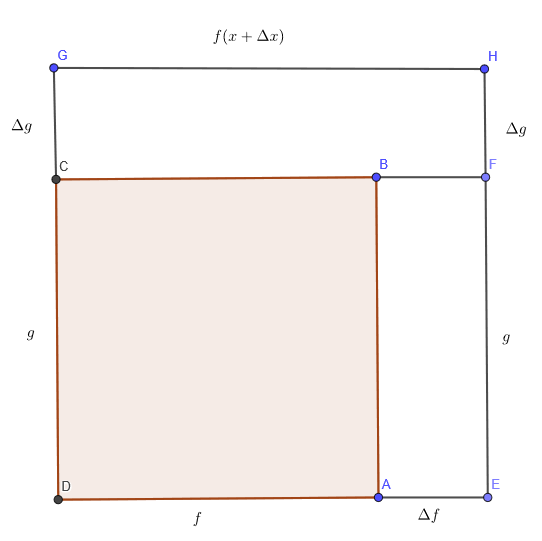
\includegraphics[scale=0.8]{Pictures/product_rule_identity.PNG}
    \caption{Illustration of $\Delta(fg)$}
    \label{fig:my_label2}
\end{figure}
The shaded area is the value of the product $fg$. By increasing the variable by a small $\Delta x$, the change of the value is represented by the un-shaded (white) region.

Hence,
\begin{align*}
    (fg)'(x)=\lim_{\Delta x\to0}\left(\dfrac{\Delta f}{\Delta x}g(x)+f(x+\Delta x)\dfrac{\Delta g}{\Delta x}\right)\\
    =f'g+fg'
\end{align*}
\end{proof}

\begin{theorem}
Suppose $f,g:\mathbb{R}\to\mathbb{R}$ are two differentiable functions such that $g\neq 0$. Then, 
$$\left(\frac{f}{g}\right)'=\dfrac{f'g-fg'}{g^2}$$
\end{theorem}
\begin{proof}
The first proof that I'm going to present here uses the product rule that we just proved, but it requires some basic knowledge about implicit differentiation.
Suppose $y(x)=\frac{f(x)}{g(x)}$, then $f(x)=y(x)g(x)$, which means \begin{align*}
    f'(x)=y'(x)g(x)+y(x)g'(x)\\
    y'(x)=\dfrac{f'(x)-y(x)g'(x)}{g(x)}\\
    y'(x)=\dfrac{f'(x)-\frac{f(x)}{g(x)}g'(x)}{g(x)}\\
    y'(x)=\dfrac{\frac{f(x)}{g(x)}g(x)-\frac{f(x)}{g(x)}g'(x)}{g(x)}\\
    y'(x)=\dfrac{f'(x)g(x)-f(x)g'(x)}{(g(x))^2}
\end{align*}
\end{proof}
\begin{proof}
The quotient rule can also be proven by first principle. The proof is left to the readers as an exercise. HaHaHa!
\end{proof}

\begin{theorem}
Suppose $f,g:\mathbb{R}\to\mathbb{R}$ are two differentiable functions such that $\operatorname{range}(f)\subseteq\operatorname{dom}(g)$, then
\[(g\circ f)'=\dfrac{dg}{df}\dfrac{df}{dx}\]
\end{theorem}
\begin{proof}
The damn argument presented in most high school materials is NOT correct, those people know nothing about the failure of their fake proof... I'm gonna tell you why...

Consider the rate of change,
\begin{align*}
    \dfrac{\Delta g}{\Delta x}=\dfrac{\Delta g}{\Delta f}\dfrac{\Delta f}{\Delta x}
\end{align*}
so that $\Delta f$ cancels out, and taking the limit gives us the desired result. NO!!! Well, it's partially correct but incomplete, damn... because of the following situation might occur:
\textbf{As $\Delta x$ goes to zero, $\Delta f$ might be equal to zero before $\Delta x$ really gets to zero}. It sounds a bit counterintuitive, but it's possible. So the first term needs to be adjusted. Here's what we should do:

We know that $g$ is differentiable at every $f(x)$ by assumption, meaning that $\frac{\Delta g}{\Delta x}=g'(f(x))+E$, where $E$ is an error term that approaches to $0$ as $\Delta x\to 0$. Thus, we should prove it by
\begin{align*}
    \dfrac{\Delta g}{\Delta x}=(g'(f(x))+E)\dfrac{\Delta f}{\Delta x}
\end{align*}
Hence,
\begin{align*}
    \lim_{\Delta x\to0}\dfrac{\Delta g}{\Delta x}=g'f'
\end{align*}
\end{proof}
This adjustment is essential even if it seems to be trivial to our readers because simply writing a quotient there makes no sense.

%Others will be included later... The reason I didn't complete them here is because 1) I need to come up with a geometric view of the quotient identity; 2) although you can derive the chain rule by cancellation, it is not rigorous enough, and an actual proof requires another parts to deal with some specific situations......

\section{The Derivative of Exponential and Logarithmic Function}
Suppose we get $e^x$, then
\begin{align*}
    \dfrac{d}{dx}e^x=\lim_{h\to 0}\dfrac{e^{x+h}-e^x}{h}\\
    =\lim_{h\to 0}\dfrac{e^x(e^h-1)}{h}\\
    =e^x\lim_{h\to 0}\dfrac{e^h-1}{h}
\end{align*}
Set $y=e^h-1$, then
\begin{align*}
    \dfrac{d}{dx}e^x=e^x\lim_{y\to0}\dfrac{y}{\ln(y+1)}
\end{align*}
Now, substituting $k=\frac{1}{y}$ will give us
\begin{align*}
    \dfrac{d}{dx}e^x=e^x\lim_{k\to\infty}\dfrac{1}{k\ln\left(\frac{1}{k}+1\right)}\\
    =e^x\lim_{k\to\infty}\dfrac{1}{\ln\left(1+\frac{1}{k}\right)^k}\\
    =e^x\dfrac{1}{\ln e}\\
    =e^x
\end{align*}

Therefore, if $f(x)=a^x$ where $a\in\mathbb{R}$, then
\[
\dfrac{d}{dx}a^x=\dfrac{d}{dx}e^{x\ln a}=\ln(a)e^{x\ln(a)}=\ln(a)a^x
\]
DONE!

Now, consider $\ln(x)$, then
\begin{align*}
    \dfrac{d}{dx}\ln(x)=\lim_{h\to 0}\dfrac{\ln(x+h)-\ln(x)}{h}\\
    =\lim_{h\to 0}\dfrac{\ln\left(\frac{x+h}{x}\right)}{h}\\
    =\lim_{h\to 0}\dfrac{\ln\left(1+\frac{h}{x}\right)}{h}\\
    =\lim_{h\to 0}\dfrac{\frac{h}{x}\ln\left(1+\frac{h}{x}\right)^{\frac{x}{h}}}{h}\\
    =\lim_{h\to 0}\left(\dfrac{1}{x}\ln\left(1+\frac{h}{x}\right)^{\frac{x}{h}}\right)\\
    =\dfrac{1}{x}\ln(e)\\
    =\dfrac{1}{x}
\end{align*}

\section{Differentiate Implicit Functions}
Before discussing any differentiation, we need to understand what is an implicit function. For this section, we only care about those functions whose graphs are visible on $\mathbb{R}^2$. It's not going to cause any confusion unless we pass to higher dimensional cases, where the graphs become some sort of manifolds...
\begin{definition}
An implicit function is defined using a relation $f(x,y)=0$
\end{definition}
\begin{example}
The unit circle can be defined by an implicit function
\[x^2+y^2-1=0\]
\end{example}
\begin{example}
Although the parabola $y=x^2$ is a function, we can also express that in implicit forms, i.e., $y-x^2=0$.
\end{example}
(Seems like an algebraic variety...)
When you want to differentiate an implicit function (if it's differentiable) then there are mainly two ways for you to do:
\begin{itemize}
    \item Convert that into different branches of explicitly defined functions. For instance we can write down the definition of a circle explicitly by $y=\pm\sqrt{1-x^2}$.
    \item Simply assume that $y$ is a function of $x$ and differentiate both side of the equation with respect to $x$.
\end{itemize}
The second method is usually the most convenient but also the most confusing. Suppose you have an implicitly defined function $f(x,y)=0$. Now, if you slightly change the value of $x$ by $h$, then to make sure that the pair $(x+h,y')$ still satisfies the equation, we need $y$ to change by a small step $h'$ also. So that $f(x+h,y+h')=0$. If not, then $f(x+h,y)\neq 0$, which will not appear on the graph. Thus, what it really means to differentiate both side is to make sure that the net change of $f(x,y)$ is always $0$. The meaning for this differentiation is to see how much $y$-coordinate needs to change when $x$-coordinate changed a really small step.
\begin{example}
We have $x^2+y^2=1$, then differentiate both side with respect to $x$ gives $2x+2y\frac{dy}{dx}=0$, so that $\frac{dy}{dx}=-\frac{x}{y}=\frac{-x}{\pm\sqrt{1-x^2}}$. To see why this gives us the slope of the tangent line for the circle at each given point $(x,y)$, consider the radius joining $(0,0)$ and $(x,y)$, its slope must be $y/x$. A simple geometry tells us that for another line $l$ to be tangent at $(x,y)$, then $l$ is perpendicular to the radius joining that point, and for this to be true, we require $m_l\frac{y}{x}=-1$, which agrees to the result of differentiation.
\end{example}
Practice more and read the following section about differentiating inverse trig functions.


\section{The Derivatives of Inverse Trigonometric Functions}
This chapter assumes that you know how to apply chain rule and the meaning of differentiating implicit functions.

The derivative of these inverse trig functions are elegant, as you'll see.

\textbf{Important note:} For the first section, you may read carefully to study the idea behind the derivation, but try to do the last two sections as exercises.
\subsection{Arcsin}
Suppose $y=\arcsin(x)$, then $x=\sin(y)$, meaning that 
\begin{align*}
    \dfrac{d}{dx}x=\dfrac{d}{dy}\sin(y)\dfrac{dy}{dx}\\
    1=\cos(y)\dfrac{dy}{dx}\\
    \dfrac{dy}{dx}=\dfrac{1}{\cos(y)}
\end{align*}
Now, substitute $\sqrt{1-x^2}=\sqrt{1-\sin^2(y)}=\cos(y)$, which yields
\[\dfrac{dy}{dx}=\dfrac{1}{\sqrt{1-x^2}}\]
You can check that the domain of this function is $[-1,1]\subset\mathbb{R}$.
\subsection{Arccos}
Suppose $y=\arccos(x)$, then $x=\cos(y)$.
\begin{align*}
    1=-\sin(y)\dfrac{dy}{dx}\\
    \dfrac{dy}{dx}=\dfrac{-1}{\sin(y)}\\
    \dfrac{dy}{dx}=-\dfrac{1}{\sqrt{1-x^2}}
\end{align*}
Do you see the relationship between the derivative of $\arcsin$ and $\arccos$?
\subsection{Arctan}
Suppose $y=\arctan(x)$, then $x=\tan(y)$.
\begin{align*}
    1=\sec^2\dfrac{dy}{dx}\\
    \dfrac{dy}{dx}=\dfrac{1}{\sec^2(x)}
\end{align*}
Use $1+\tan^2(y)=\sec^2(y)$ to rewrite the equation above as
\[\dfrac{dy}{dx}=\dfrac{1}{1+x^2}\]
\textbf{Question:} Can you guess answer to $\frac{d}{dx}\cot^{-1}(x)$? Justify your answer with rigorous argument.

\subsection{Bonus Section!}
We're going to differentiate $\sec^{-1}(x)$ and $\csc^{-1}(x)$!

Suppose $y=\sec^{-1}(x)$, then $x=\sec(y)$.
\begin{align*}
    1=\sec(y)\tan(y)\dfrac{dy}{dx}\\
    \dfrac{dy}{dx}=\dfrac{1}{\sec(y)\tan(y)}
\end{align*}
Here it becomes a bit tricky. The domain of $\sec^{-1}(x)$ is $(-\infty,-1]\cup[1,\infty)$, so the range should be $[0,\pi/2)\cup(\pi/2,\pi]$. Hence, 
\[
\tan(y)=
\begin{cases}
\sqrt{x^2-1} & x\ge 1\\
-\sqrt{x^2-1} & x\le -1
\end{cases}
\]
Therefore,
\[\dfrac{d}{dx}\sec^{-1}(x)=\dfrac{1}{|x|\sqrt{x^2-1}}\]

We turn to $\csc^{-1}(x)$ now.
Suppose $y=\csc^{-1}(x)$, then
\begin{align*}
    \dfrac{dy}{dx}=-\dfrac{1}{\csc(y)\cot(y)}
\end{align*}
Again, 
\[
\cot(y)=\begin{cases}
-\sqrt{x^2-1} & x\ge 1\\
\sqrt{x^2-1} & x\le -1
\end{cases}
\]
similarly for $\csc(y)$...
Hence, one has
\[\dfrac{d}{dx}\csc^{-1}(x)=-\dfrac{1}{|x|\sqrt{x^2-1}}\]

\section{Differentiability and Continuity}
\begin{theorem}
Differentiability implies continuity.
\end{theorem}
\begin{proof}
Suppose $f:\mathbb{R}\to\mathbb{R}$ is differentiable, then $\lim_{\Delta x\to0}\frac{\Delta f}{\Delta x}=N<\infty$. Hence, if $\Delta f\not\to 0$, then the whole limit would blow up, so we know that $\Delta f\to 0$ as $\Delta x\to 0$. This is basically what the definition of continuity says.
\end{proof}
\begin{theorem}
The converse of the preceding claim doesn't hold.
\end{theorem}
\begin{proof}
There is an simple but "philo" counterexample. Consider Thomae's Function, which is defined as
\[
T(x)=\begin{cases}
\dfrac{1}{q} & x=\dfrac{p}{q}, \operatorname{gcd}(p,q)=1\\
0 & \text{Otherwise}
\end{cases}
\]
I claim without proof that $T(x)$ is continuous on $\mathbb{R}\setminus\mathbb{Q}$ (continuous at every irrational number) but it's nowhere differentiable.
\end{proof}
Google "Thomae's Function" for more information.

\section{L'Hopital's Rule}
\begin{theorem}
Suppose $f,g:\mathbb{R}\to\mathbb{R}$ are two differentiable functions, then if \textbf{either} 
\[\dfrac{f(x)}{g(x)}=\dfrac{0}{0}\text{ OR }\dfrac{f(x)}{g(x)}=\dfrac{\pm\infty}{\pm\infty}\]
then 
\[\lim_{x\to c}\dfrac{f(x)}{g(x)}=\lim_{x\to c}\dfrac{f'(x)}{g'(x)}\]
provided that the limit of the second term exists.
\end{theorem}
Here are some examples of applications of L'Hopital's rule.
\begin{example}
The limit of ational functions using L'Hopital's rule:
\[
\lim_{x\to\infty}\dfrac{ax+b}{cx+d}=\lim_{x\to \infty}\dfrac{a}{c}=\dfrac{a}{c}
\]
Using standard method,
\[
\lim_{x\to\infty}\dfrac{ax+b}{cx+d}=\lim_{x\to \infty}\dfrac{a+\frac{b}{x}}{c+\frac{d}{x}}=\dfrac{a}{c}
\]
\end{example}
\begin{exercise}
The example above demonstrates how to manipulate the limit of the quotient of two linear function. Consider the quotient of two polynomial. Can you deduce a general result of the limit using L'Hopital's rule? (Remember! L'Hopital's rule can be applied repetitively.)
\end{exercise}
\begin{example}
Consider $\lim_{x\to -\infty}xe^x$. This function does not have the form of a quotient, and the limit looks like $-\infty\times 0$, which implies nothing. However, this does not imply that the limit is unsolvable. Our goal is to rewrite the expression in quotient form and apply L'Hopital's rule.

Let's try this
\[L=\lim_{x\to-\infty}\dfrac{e^x}{1/x}\]
Apply L'Hopital's rule,
\[
L=\lim_{x\to-\infty}\dfrac{e^x}{-1/x^2}=\lim_{x\to-\infty}\dfrac{e^x}{2/x^3}=\ldots
\]
which gives us nothing, so let's try the other way.
\[L=\lim_{x\to-\infty}\dfrac{x}{e^{-x}}=\lim_{x\to-\infty}\dfrac{1}{-e^{-x}}=0\]
\end{example}
\begin{example}
Consider $$S=\lim_{x\to 0^+}(x^2\ln^2(x))$$ then
\[
S=\lim_{x\to0^+}\dfrac{\ln^2(x)}{x^2}=\lim_{x\to 0^+}\dfrac{2\ln(x)\frac{1}{x}}{-2/x^2}=\lim_{x\to 0^+}\dfrac{\ln(x)}{-1/x}=\lim_{x\to 0^+}\dfrac{1/x}{1/x^2}=\lim_{x\to 0^+}x=0\]
\end{example}
\begin{example}
When there is a product, you should attempt to rewrite it as a quotient in order to apply L'Hospital's rule. Remember that your intuition plays a very important role.
\[
\lim_{x\to\infty}x\sin\left(\dfrac{7}{x}\right)=\lim_{x\to\infty}\dfrac{\sin(7/x)}{1/x}=\lim_{x\to\infty}\dfrac{\cos(7/x)\frac{-7}{x^2}}{-1/x^2}=\lim_{x\to\infty}7\cos(7/x)=7
\]
\end{example}

These two examples show that practice is really important. The following two examples will demonstrate the techniques of using logarithmic function to evaluate the limit, which is usually applied to an exponential form.
\begin{example}
Consider
\[
y=\lim_{t\to 0^+}(e^t+t)^{1/t}
\]
This does not belong to any familiar form of expression, but since there is an exponent, we can use logarithmic function to "pull it down".
\[
\ln(y)=\lim_{x\to 0^+}\dfrac{e^t+t}{t}=\lim_{x\to 0^+}\dfrac{e^t+1}{1}=2
\]
So, $y=e^{\ln(y)}=e^2$, meaning that the limit is $e^2$.
\end{example}
\begin{example}
Suppose $z=\lim_{x\to \infty}(e^{-2t}+3t)^{1/t}$, then
\[
\ln(z)=\lim_{x\to \infty}\dfrac{e^{-2t}+3t}{t}=\lim_{x\to\infty}\dfrac{-2e^{-2t}+3}{1}=3
\]
Therefore, the limit is $z=e^3$.
\end{example}
We've already seen some tricks of manipulating expressions, but in some cases, you need to apply L'Hospital's rule multiple times (usually, 1 to 2 times is enough).
\begin{example}
Consider
\begin{align*}
\lim_{y\to\infty}\dfrac{y^2-e^{6y}}{4y^2+e^{7y}}\\
=\lim_{y\to\infty}\dfrac{2y-6e^{6y}}{8y+7e^{7y}}\\
=\lim_{y\to\infty}\dfrac{2-36e^{6y}}{8+49e^{7y}}\\
=\lim_{y\to\infty}\dfrac{-216e^{6y}}{343e^{7y}}\\
=\lim_{y\to\infty}\dfrac{-216}{343e^y}\\
=0
\end{align*}
There is an example in Haese textbook that shows how to find the limit of $\dfrac{e^x}{x^n}$. Take a look at it.
\end{example}

\textbf{Acknowledgement: Most exercises in this section are from Professor Paul's Notes on} \url{https://tutorial.math.lamar.edu/ProblemsNS/CalcI/LHospitalsRule.aspx}

\section{Taylor Series}
This is a method to approach a function using polynomials. I'll first give the definition and discuss why it's like that.
\begin{definition}
Suppose $f:(a,b)\to\mathbb{R}$ is continuously differentiable at $x=c$ (the derivatives of all degree exists for $x=c$), then the Talor series of $f$ at $c$ is
\[
\sum_{m=0}^\infty\dfrac{f^{(m)}(c)}{m!}(x-c)^m
\]
There is an important quantity to be considered, which is the remainder $R_n$ defined as
\[
R_n(x)=f(x)-\sum_{m=0}^{n-1}\dfrac{f^{(m)}(c)}{m!}(x-c)^m
\]
\end{definition}
The term $R_n$ is an error term that measure how close is the original function $f$ and the polynomial approximation. If $R_n$ tends to zero as $n\to \infty$, then we say that $f(x)=\sum_{m=0}^\infty\dfrac{f^{(m)}(c)}{m!}(x-c)^m$ (vice versa).

There's always a question at this point: Why is that power series approximate $f$? Here is the answer.
Consider a power series
\[f(x)=\sum_{m=1}^\infty a_mx^m\]
such that $f$ converges for $|x|<R$, where $R$ is the radius of convergence, then because this power series is NICE when $|x|<R$, we can differentiate it term by term, i.e.,
\[\dfrac{d}{dx}f(x)=\dfrac{d}{dx}\sum_{m=1}^\infty a_mx^m=\sum_{m=1}^\infty\dfrac{d}{dx} a_mx^m\]
\textbf{Your task is to observe the pattern for $f'$, $f''$, $f'''$ and conclude what is $f^{(l)}$.} (This is your task because I'm lazy...)

Answer:
\[
f^{(l)}(x)=\sum_{m=l}^\infty m(m-1)...(m-l+1)a_mx^{m-l}
\]
Substitute $x=0$ gives you a factorial. To offset the impact of differentiating (because it keeps changing the coefficient), we need to divide each term by $m!$. Hence,
\[f(x)=\sum_{m=0}^\infty\dfrac{f^{(m)}(c)}{m!}(x-c)^m\]

Another potential problem: What is the difference between Taylor Series and Maclaurin Series? Well, the difference is subtle because Taylor series refers to the series expansion of a function at some point in its domain, whereas Maclaurin series refers to the Taylor series at $x=0$.

\subsection{Taylor Series of Trigonometric Functions (Incomplete)}
We start by looking at the Maclaurin series of $\sin(x)$.

At $x=0$, $\sin(x)=0$ meaning that the constant term of its expansion is also zero. $(\sin(0))'=\cos(0)=1$ shows that the degree $1$ term of its expansion is $1$. $(\sin(0))''=-\sin(0)=0$, so the quadratic term must be zero. In other words there's no proper quadratic approximation for $\sin(x)$ at $x=0$. Then, we have $(\sin(0))'''=-\cos(0)=-1$, meaning that the coefficient for the cubic term is $\frac{-1}{3!}$. Repeat this process, you'll see that 
\[\sin(x)=0+x+0x^2-\dfrac{1}{3!}x^3+0x^4+\frac{1}{5!}x^5+\ldots\]
Hence,
\begin{align*}
    \sin(x)=\sum_{m=0}^\infty\dfrac{(-1)^n}{(2m+1)!}x^{2m+1}
\end{align*}
This also shows that $\sin(x)$ is an odd function (connect to what Karbro said).

Then, we're going to look at $\cos(x)$.

The process is similar, so it will be left to the readers to complete. (I'm lazy...)
\[
\cos(x)=1+0x-\dfrac{1}{2!}x^2+0x^3+\dfrac{1}{4!}x^4+\ldots
\]
which means
\[
\cos(x)=\sum_{m=0}^\infty\dfrac{(-1)^m}{(2m)!}x^{2m}
\]

\subsubsection{Challenge}
Can you derive the Maclaurin sereis of $\tan(x)$, $\sec(x)$, $\csc(x)$, and $\cot(x)$? I can't..... :(

\subsubsection{Answer to the challenge}
:) 

Suppose $\tan(x)=\sum_{m=0}^\infty a_mx^m$, then
\begin{enumerate}
    \item $\tan(0)=0$ implies $a_0=0$;
    \item $(\tan(0))'=\sec^2(0)=1$ implies $a_1=1$;
    \item $(\tan(0))''=0$ implies $a_2=0$;
    \item $(\tan(0))'''=6\sec^4(0)-4\sec^2(0)=2$ implies $a_3=2/6$;
    \item ......
\end{enumerate}
So, 
\[
\tan(x)=x+\dfrac{1}{3}x^3+\dfrac{2}{15}x^5+\ldots
\]
I'm not sure how to rewrite this using sigma notation...... :(

\subsection{Taylor Series of Exponential and Logarithmic Function}
A simple fact allows us to conclude the Maclaurin series of $e^x$ really quickly. Note that $\frac{d}{dx}e^x=e^x$, so
\[
e^x=1+x+\dfrac{1}{2!}x^2+\ldots=\sum_{m=0}^\infty\dfrac{1}{m!}x^m
\]

Now, for logarithmic function, we only care about the natural log because we can always change the base. However, $\ln(x)$ is undefined at $x=0$ so we're going to consider $\ln(x+1)$ and derive its Maclaurin series. Suppose $\ln(1+x)=\sum_{m=0}^\infty b_mx^m$, then
\begin{enumerate}
    \item $\ln(0+1)=0$ implies $b_0=0$;
    \item $(\ln(0+1))'=\frac{1}{0+1}=1$ implies $b_1=1$;
    \item $(\ln(0+1))''=-\frac{1}{(0+1)^2}=-1$ implies $b_2=-\frac{1}{2!}$;
    \item $(\ln(0+1))'''=2\dfrac{1}{(0+1)^3}=2$ implies $b_3=\frac{2}{3!}$;
    \item ......
    \item $(\ln(0+1))^{(k)}=(-1)^{k+1}(k-1)!$ implies $b_k=\frac{(-1)^{k+1}(k-1)!}{k!}=\frac{1}{k}$;
\end{enumerate}
So,
\[
\ln(1+x)=\sum_{m=1}^\infty\dfrac{(-1)^{m+1}}{m}x^m=\sum_{m=0}^\infty\dfrac{(-1)^m}{(m+1)}x^{m+1}
\]

\subsection{Proof of De Moivre's Theorem}
We learned in the chapter of complex number that $e^{ix}=\cos(x)+i\sin(x)$. We're going to give a proof using Maclaurin series.
\begin{proof}
\begin{align*}
    e^{ix}=\sum_{m=0}^\infty\dfrac{1}{m!}(ix)^m\\
    =1+ix+\dfrac{1}{2}i^2x^2+\dfrac{1}{3!}i^3x^3+\ldots\\
    =1+ix-\dfrac{1}{2}x^2-i\dfrac{1}{3!}x^3+\dfrac{1}{4!}x^4+\ldots\\
    =\left(1-\dfrac{1}{2!}x^2+\dfrac{1}{4!}x^4+\ldots\right)+i\left(x-\dfrac{1}{3!}x^3+\dfrac{1}{5!}x^5+\ldots\right)\\
    =\cos(x)+i\sin(x)
\end{align*}
\end{proof}

\subsection{Typical Questions}
Given an aribitrary analytic function $f:\mathbb{R}\to\mathbb{R}$ and the $n$-th degree taylor polynomial of $f$ at $x=0$ is given by $p(x)$. Then, you should know the value for $f^{(k)}(0)$ for $k\le n$.

\section{Integration}
The author assumes that the readers know all basic anti-derivatives. To check whether you can adroitly apply them, consider the following lists of questions, give yourself 10 seconds to answer each question. If you can do it, then congrats, you may advance to the next paragraph.
\textbf{State the indefinite integral of all the following functions}
\begin{enumerate}
    \item $ax^b$
    \item $\sin(x)$
    \item $\cos(x)$
    \item $a\sin(x)$
    \item $a\cos(x)$
    \item $\sec^2(x)$
    \item $-\csc^2(x)$
    \item $e^x$
    \item $1/x$
\end{enumerate}

However, when the function is more complicated, we need some more advanced techniques to figure out the answer.

\subsection{Integration by substitution}
The strategy is really simple. Suppose we have a continuous function $h:\mathbb{R}\to\mathbb{R}$ that is of the form $h(x)=f(x)f'(x)$, and we want to integrate with respect to $x$, meaning that
\[
\int h(x)dx=\int f(x)f'(x)dx
\]
If we substitute a new variable $u=f(x)$, then $du=f'(x)dx$, which turns this integral into
\[
\int udu
\]
(integrating with respect to $u$) Although after you you figure out what to substitute and how to substitute, the integral becomes fairly easy, you still need lots of practice in order to get a kind of intuition, i.e., you need to perceive that there exists a function $f$ and its derivative $f'$ in the integrand.Whenever you see some "complicated structure" in the integrand, if it is a polynomial of degree $n$, then you may want to substitute it as $u$ if there is a polynomial of degree $n-1$ outside of that structure. 
\begin{example}
We should substitute $u=x^2+1$ in the following case.
\[
\int x\sqrt{x^2+1}dx
\]
which then becomes
\[
\int \dfrac{1}{2}\sqrt{u}du
\]
because $du=2xdx$, so we multiply a factor of $1/2$ to eliminate the effect of $2$.
\end{example}

Also, make that you can sense the existence of the derivative of natural log.
\begin{example}
Consider \[\int\dfrac{\ln(x)}{x}dx\] By substituting $u=\ln(x)$, the integral actually becomes \[\int udu\]
\end{example}

\subsubsection{Trigonometric Substitution}
What the author (I) found sometimes difficult is trigonometric substitution because it requires a quite adroit manipulation of trigonometric identities.
\begin{example}
Consider \[I=\int\dfrac{dx}{\sqrt{1-x^2}}\] If you can write the answer down in two seconds, then this example is not for you because you already master the differentiation of inverse trigonometric functions. (Congratulations!) Suppose you don't the answer, but you know the strategy is substitution. The most obvious two are probably $\sqrt{1-x^2}$ and $1-x^2$, but in either case $du$ makes the expression really ugly, so don't do it. Instead, you should think about how to get rid of the square root sign. Here, the identity $\sin^2(\theta)+\cos^2(\theta)=1$ does a great job. Let's see. Substitute $x=\sin(\theta)$, so that 
\[
I=\int\dfrac{dx}{\sqrt{1-\sin^2(\theta)}}
\]
We also need something to replace $dx$, but it's easy because $x=\sin(\theta)\implies dx=\cos(\theta)d\theta$. So,
\[
I=\int\dfrac{\cos(\theta)d\theta}{\cos(\theta)}=\int d\theta=\theta+C=\arcsin(x)+C
\]
\end{example}

\begin{exercise}
Find the following indefinite integrals by trigonometric substitution.
\begin{enumerate}
	\item $\int \dfrac{dx}{1+x^2}$
	\item $\int \dfrac{-dx}{\sqrt{1-x^2}}$
\end{enumerate}
\end{exercise}

Now comes a challenge.
\begin{example}
We want to find \[I=\int \dfrac{dx}{\sqrt{1+x^2}}\]
It is tempting to substitute sine or cosine in to the expression because this is similar to the previous example,but no, we use $x=\tan(\theta)$ because $1+\tan(\theta)=\sec^2(\theta)$ completes the square.After a series of manipulation,
\[
I=\int\sec(\theta)d\theta=\ln|\sec(\theta)+\tan(\theta)|+C=\ln|\sec(\arctan(x))+x|+C
\]
The integration of secant function is in the textbook (Pearson). Do check it out.
\end{example}

The strategy of substituting trigonometric terms doesn't only work for $x$ but actually in general. Whenever there is a square root sign or things like $1+[f(x)]^2$ in the denominator, we always try to substitute trig terms to simplify it. Here is a sample question from Pearson's textbook.
\begin{example}
We want to find \[ \int \dfrac{e^{-2x}dx}{\sqrt{1-e^{-4x}}}\]
Now, substitute $e^{-2x}=\sin(\phi)$, then $dx=\frac{\cos(\phi)d\phi}{-2e^{-2x}}$, which implies that $e^{-2x}dx=-\frac{1}{2}\cos(\phi)d\phi$. Thus, the integral turns out to be
\[
-\dfrac{1}{2}\int\dfrac{\cos(\phi)d\phi}{\cos(\phi)}=-\dfrac{1}{2}\phi+C=-\dfrac{1}{2}\arcsin(e^{-2x})+C
\]
\end{example}

We want to generalize these trigonometric substitution as follows.
\begin{example}
    Consider
    \[
    I=\int \dfrac{dx}{\sqrt{a^2-x^2}}    
    \]
    We know that $a^2\sin^2(\theta)+a^2\sin^2(\theta)=a^2$, so we'll substitute $x=a\sin\theta$ to obtain
    \[
    \int\dfrac{a\cos\theta d\theta}{a\cos\theta}=\int d\theta=\arcsin\left(\dfrac{x}{a}\right)+C    
    \]
    If we remove the square root sign, then this substitution still works because the denominator becomes $a^2\cos^2(\theta)$, and this is a simple integral that we can solve.
    If there is a minus sign in the integrand, then we usually substitute $\cos(\theta)$ because its derivative contains a minus sign to cancel out the minus sign in the integrand.
\end{example}
\begin{example}
    Now, we consider another class of integral
    \[
        I=\int\dfrac{dx}{a^2+x^2}
    \]
    In this case, we usually consider substituting $x=a\tan(\theta)$ because the identity $a^2+a^2\tan^2(x)=a^2\sec^2(x)$ will convert the sum in the denominator to a monomial.
    Thus,
    \[I=\int \dfrac{a\sec^2\theta d\theta}{a\sec^2\theta}=\int d\theta=\theta+C=\dfrac{1}{a}\tan\left(\dfrac{x}{a}\right)+C\]
    If we add a square root sign on the denominator, then we can also substitute tangent function. The only difference is that the denominator will become $a\sec(x)$.
\end{example}

You also need to anticipate the existence of constant in your substitution. If $I=\int x\sqrt{9-x^2}$, then you can substitute $u=x^2$, but it still leaves you with the term $\sqrt{9-u}$,
which is not good, but because the derivative of a constant vanishes, you can always use $u=9-x^2$, and this helps you make progress.
Also, you need to be able to identify the relationship between derivative and anti-derivative. For instance, test if you can identify what to substitute in $\int\frac{\csc(x)\cot(x)}{3-\csc(x)}dx$.
If you can't do it in two seconds, then you really need more practice (sry). Sometimes, the substitution is really complex. Don't be shocked or intimidated by the complex structure of the integrand.
\begin{example}
    Consider the integral
    \[I=\int(\sin(3x)-x^3)^5(\cos(3x)-x^2)dx\]
    The correct substitution is $u=\sin(3x)-x^3$.
\end{example}
\begin{example}
    For this one,
    \[4\int\left(\dfrac{1}{x}-e^{-x}\right)\cos(e^{-x}+\ln(x))dx\]
    You use $u=e^{-x}+\ln(x)$.
\end{example}
\begin{example}
    For $$\int\dfrac{e^{\tan(x)}}{\cos^2(x)}$$
    try substituting $u=\tan(x)$. You should be able to justify this substitution immediately.
\end{example}

\subsubsection{Definite integration}
Consider \[I=\int_a^b f(x)dx\]
we want to use substitution $u=g(x)$ so that $du=g'(x)dx$. Then, 
\[I = \int_{x=a}^{x=b}f(g(x))g'(x)dx = \int_{x=a}^{x=b}f(u)du = \int_{g(a)}^{g(b)}f(u)du\]
The reason for changing the parameter is because we want to integrate with respect to the variable $u$, which is determined by $x$.

\subsection{Integration by part}
We start by an example. Consider the indefinite integral
\[
\int xe^xdx
\]
In this case,there is no way to use substitution. For example, if substitute $u=x$, then it's basically useless. On the other hand, if you try substitute $u=e^x$, then $x=\ln(u)$, which is no good either. So, probably integration by substitution is not a good idea to do this one.

Think about the rules of differentiation and that integration is the reversed operation of differentiation. Substitution corresponds to undo the effect of chain rule. Can we reverse the product rule? Well, yes.

Suppose we have a product $f(x)=u(x)v(x)$ such that $f$ is differentiable, then by the product rule, we have 
\[\dfrac{d}{dx}(uv)=u\dfrac{dv}{dx}+v\dfrac{du}{dx}\]
Now, we take the integral on both side
\[
\int \dfrac{d}{dx}(uv)dx=\int u\dfrac{dv}{dx}dx+\int v\dfrac{du}{dx}dx=\int udv+\int vdu
\]
Let's rearrange the equation, we found that 
\[
\int udv=uv-\int vdu
\]
This gives the formula for integration by parts, which says that if the integrand has the form $udv$, then you can find the indefinite integral by setting proper $u$ and proper $dv$ to convert the integral into something you know about. Now, let's return to the example $xe^x$.

Let's try setting $u=e^x$ and $dv=xdx$. Then, $du=e^xdx$ and $v=\frac{1}{2}x^2$, which means
\[
\int xe^xdx=\dfrac{1}{2}x^2e^x-\dfrac{1}{2}\int x^2e^xdx
\]
Ooops! We don't know the integral of $x^2e^x$ yet, and that thing actually needs another integration by parts, which is not so convenient, so let's try the other way.

Let $u=x$ and $dv= e^xdx$, then $du=dx$ and $v=e^x$. Therefore, we have
\[
\int xe^xdx=xe^x-\int e^xdx=xe^x-e^x+C
\]
DON'T FORGET THE ARBITRARY CONSTANT!

Sometimes, the two integrands are not obvious at all, so you might need to invoke $dv=dx$ in order to proceed integration by parts.
\begin{example}
    Consider
    \[I=\int\sin(\ln(x))dx\]
    If you try any kind of substitution, you will fail. Meanwhile, this function is not a product, so it's time to invoke $u=\sin(\ln(x))$ and $dv=dx$!
    Using integration by parts, we get
    \[
    I = x\sin(\ln(x))-\int x\cos(\ln(x))\dfrac{dx}{x}=x\sin(\ln(x))-\int\cos(\ln(x))dx    
    \]
    which is really nice. Now, use integration again (the same strategy), one can obtain
    \[
    I=x\sin(\ln(x))-x\cos(\ln(x))+\int -x\sin(\ln(x))\dfrac{dx}{x}= x\sin(\ln(x))-x\cos(\ln(x))-\int x\sin(\ln(x))dx 
    \]
    Therefore,
    \[I=\dfrac{x\sin(\ln(x))-x\cos(\ln(x))}{2}+C\]
\end{example}

\begin{example}
    We try to prove an identity in this example. Suppose $f:[a,b]\to\mathbb{R}$ is twice differentiable and its second derivative $f''$ is Riemann integrable, then we have
    \[\int_a^b f(x)dx = \dfrac{(b-a)(f(a)+f(b))}{2}+\dfrac{1}{2}\int_a^b f''(x)(x-a)(x-b)dx\]
    We want to use integration by parts because of the form of the right hand side. So, set $u=f(x)$, $dv=dx$, we get
    \[
    \int_a^b f(x)dx = [xf(x)]_a^b-\int_a^b xf'(x)dx=bf(b)-af(a)-\int_a^b xf'(x)dx
    \]
    %Use integration by parts again to obtain
    %\[\int_a^b xf'(x)dx = [\dfrac{1}{2}x^2f'(x)]_a^b-\dfrac{1}{2}\int_a^b x^2f''(x)dx = \dfrac{1}{2}(a^2f'(a)-b^2f'(b))\]
    Now, we approach this question from the right hand side.
    The integral at then end can be written as
    \[
        \dfrac{1}{2}\int_a^b f''(x)(x-a)(x-b)dx=-\dfrac{1}{2}\int_a^bf'(x)(2x-a-b)dx    
    \]
    using integration by part with $u=(x-a)(x-b)$ and $dv=f''(x)dx$. Moreover, we have
    \begin{align*}
        -\dfrac{1}{2}\int_a^bf'(x)(2x-a-b)dx=-\dfrac{1}{2}\left(\int_a^b 2xf'(x)dx-(a+b)\int_a^b f'(x)dx\right)\\
        =-\int_a^b xf'(x)dx+\dfrac{af(b)+af(a)+bf(b)-bf(a)}{2}
    \end{align*}
    Therefore,
    \begin{align*}
        \dfrac{(b-a)(f(a)+f(b))}{2}+\dfrac{1}{2}\int_a^b f''(x)(x-a)(x-b)dx= \dfrac{(b-a)(f(a)+f(b))}{2}-\dfrac{1}{2}\int_a^bf'(x)(2x-a-b)dx\\
        =\dfrac{bf(a)+bf(b)-af(a)-af(b)}{2}+\dfrac{af(b)-af(a)+bf(b)-bf(a)}{2}-\int_a^b xf'(x)dx\\
        =bf(b)-af(a)-\int_a^b xf'(x)dx\\
        =\int_a^b f(x)dx
    \end{align*}
    which completes the proof
\end{example}

Note, even though integration by parts is a really strong tool for finding the anti-derivative, it is still limited. Functions like the following one cannot be evaluated using any method that is covered so far.
\[I=\int\dfrac{\cos(x)}{x}dx\]
This integral is often denoted $Ci(x)$, but you can write down the anti-derivative using power series, which will be introduced later.

\subsubsection{Induction Method}
There might exist some questions that ask you to prove an integral formula by induction, in which case integration by parts will be an essential tool. Here are some questions that I found online.
\subsection{Reduction formula}
Here, I'll derive the reduction formula for the powers of trigonometric functions.
\begin{align*}
    \int\sin^nxdx=\int\sin^{n-1}x\sin xdx=-\cos(x)\sin^{n-1}(x)-(n-1)\int-\cos^2(x)\sin^{n-1}(x)dx\\
    = -\cos(x)\sin^{n-1}(x)+(n-1)\int\sin^{n-2}(x)(1-\sin^2(x))dx\\
    = -\cos(x)\sin^{n-1}(x)+(n-1)\int\sin^{n-2}(x)dx-(n-1)\int\sin^n(x)dx\\
    = -\dfrac{1}{n}\cos(x)\sin^{n-1}(x)+\dfrac{n-1}{n}\int\sin^{n-2}(x)dx
\end{align*}

The reduction formula for cosine was discussed in class, so I'll skip that. haha\dots

\begin{align*}
    \int\csc^n(x)=\int\csc^{n-2}(x)\csc^2(x)dx\\
    =-\cot(x)\csc^{n-2}(x)-(n-2)\int -\cot^2(x)\csc^{n-2}(x)dx\\
    =-\cot(x)\csc^{n-2}(x)-(n-2)\int\csc^{n-2}(x)(\csc^2(x)-1)dx\\
    =-\dfrac{1}{n-1}\cot(x)\csc^{n-2}(x)+\dfrac{n-2}{n-1}\csc^{n-2}(x)dx
\end{align*}

\subsection{Volume of Revolution}
\subsection{Foundation}
Given a continuous function $f(x)$ over an interval $[a,b]$,
we want to find the volume obtained by rotating the area bounded by $f(x)$, $x=a,\ x=b,\ y=0$ with respect to the $x$-axis.

Suppose we have a partition $P=\{a=x_0<x_1<\ldots<x_n=b\}$ of the interval $[a,b]$.
Clearly, we have 
\[
\sum_{i=1}^n\pi m_i^2(x_{i}-x_{i-1})\le V\le \sum_{i=1}^n M_i(x_{i}-x_{i-1})   
\]
Take the limit of upper sum and lower sum and apply squeeze lemma, we know that
\[
V=\int_a^b\pi f(x)^2dx    
\]
There are some tricky integrand related to this kind of integrals. 
\begin{example}
    Consider $$\pi\int_1^e(\ln x)^2dx$$. We use integration by parts to get
    \begin{align*}
        &\pi\int_1^e(\ln x)^2dx=\pi([x\ln^2 x]_1^e-2\int_1^e x\ln x\dfrac{1}{x}dx)\\
        &=\pi([x\ln^2 x]_1^e-2\int_1^e \ln xdx)\\
        &=\pi(e-2)
    \end{align*}
    Remember that $\int\ln xdx=x\ln x-x+C$!
\end{example}

\subsection{Improper Integral}
Let $f:[a,\infty)\to\RR$ be a real-valued function. If $\int_a^b f(x)dx$ exists for all $b>a$, and $\lim_{b\to\infty}\int_a^b f(x)dx$ exists,
then we define the improper integral to be
$$\int_a^\infty f(x)dx:=\lim_{b\to\infty}\int_a^b f(x)dx$$
\begin{remark}
    Note that if $f:[a,\infty)\to\RR$ is continuous, then $\int_a^b f(x)dx$ automatically exists for all $b>a$.
\end{remark}
\begin{example}
    An example of convergent improper integral.
    \[
    \int_1^\infty\dfrac{dx}{x^2}=\lim_{b\to\infty}\dfrac{dx}{x^2}=\lim_{b\to\infty}\left[\dfrac{-1}{x}\right]_1^b=0-(-1)=1
    \]
\end{example}
\begin{example}
    An example of divergent improper integral.
    \[
    \int_1^\infty\dfrac{dx}{x}=\lim_{b\to\infty}\int_1^b\dfrac{dx}{x}=\lim_{b\to\infty}[\ln(x)]_1^b=\infty    
    \]
\end{example}
\begin{example}
    An example of undefined improper integral
    \[
    \int_0^\infty\cos xdx    
    \]
    The reason is that $\lim_{x\to\infty}\sin(x)$ doesn't exist...
\end{example}
\subsubsection{p-integrals}
$p$-integrals refer to the following class of improper integrals.
\[
\int_1^\infty\dfrac{dx}{x^p}    
\]
\begin{theorem}
    $\int_1^\infty\frac{dx}{x^p}$ converges if $p>1$ and diverges if $0<p\le 1$. For negative exponents, there is a similar result. The readers can state and prove by themselves
\end{theorem}
\begin{proof}
    Suppose $p=1$, then the integral diverges (one of our example). Suppose $0<p\le 1$, then $\frac{1}{x^p}\ge \frac{1}{x}$, which implies that the integral diverges.
    If $p>1$, then we have 
    \begin{align*}
        &\int_1^\infty\dfrac{dx}{x^p}=\lim_{b\to\infty}\int_1^b\dfrac{dx}{x^p}\\
        &=\lim_{b\to\infty}\left[\dfrac{1}{-p+1}x^{-p+1}\right]_1^b=\lim_{b\to\infty}\left(\dfrac{1}{-p+1}b^{-p}-\dfrac{1}{-p+1}\right)\\
        &=\dfrac{1}{1-p}<\infty
    \end{align*}
\end{proof}
\begin{theorem}
    $\int_0^1x^pdx$ converges if $p>-1$.
\end{theorem}
\begin{proof}
    Let $p>-1$, we have
    \begin{align*}
        &\int_0^1x^pdx=\lim_{c\to 0}\int_c^1x^pdx\\
        &=\lim_{c\to0}\left[\dfrac{1}{p+1}x^{p+1}\right]_c^1\\
        &=\lim_{c\to0}\left(\dfrac{1}{p+1}-\dfrac{c^{p+1}}{p+1}\right)\\
        &=\dfrac{1}{p+1}
    \end{align*}
\end{proof}
The converse of the theorems above are left to the readers.
\subsection{Tricky part}
When evaluating integrals of the form $\int_{-\infty}^\infty f(x)dx$,
we need to check the convergence of $\int_a^\infty f(x)dx$ and $\int_{-\infty}^a f(x)dx$.
This is not equivalent to checking the existence of $\lim_{b\to\infty}\int_{-b}^b f(x)dx$.
\section{Differential Equation}
\subsection{Variable Separation}
\subsection{Homogeneous first order ODE}
\subsection{Non-homogeneous first order ODE}
\subsection{Seoncond Order ODE (bonus section)}
\section{Geometry}
We are working in the Euclidean space!!!
\subsection{Dot Product}
Suppose $\vec{p},\vec{q}\in\RR^n$, then their dot product inside
\[
\vec{p}\cdot\vec{q}=\begin{bmatrix}
    p_1\\p_2\\p_3\\ \vdots\\p_n
\end{bmatrix}\cdot\begin{bmatrix}
    q_1\\q_2\\q_3\\ \vdots\\q_n
\end{bmatrix}  
=\sum_{i=1}^n p_iq_i 
\]
A very important equation to be kept in mind is 
\[\vec{p}\cdot\vec{q}=\Vert p\Vert\Vert q\Vert\cos\theta\]
where $\theta$ is the angle between the two vectors.
\subsection{Cross Product}
In $\RR^3$, there is a reason for defining the cross product! We want to be able to find a third vector perpendicular to the given two! Here is the derivation, which I'll complete later.
\subsection{Distance}
It means what it means.
\subsubsection{Lines}
For two parallel lines that do not coincide. Suppose 
\begin{align*}
    &l_1:\vec{p_1}+\lambda_1\vec{d_1}\\
    &l_2:\vec{p_2}+\lambda_2\vec{d_2}
\end{align*}
\[
D=\left\Vert(\vec{p_2}-\vec{p_1})\times \dfrac{(\vec{p_2}-\vec{p_1})\cdot \vec{d_1}}{\Vert d_1\Vert^2}\vec{d_1}\right\Vert   
\]
Suppose $l_1$ and $l_2$ are skewed, i.e., $\vec{d_1}\times\vec{d_2}\neq 0$, then
\[
D=\dfrac{\vert(\vec{p_2}-\vec{p_1})\cdot(\vec{d_1}\times\vec{d_2})\vert}{\Vert\vec{d_1}\times\vec{d_2}\Vert}    
\]
\subsubsection{Line and Plane}
Suppose 
\begin{align*}
    &l:\vec{p}+\lambda\vec{d}\\
    &\Pi:ax+by+cz=d
\end{align*}
Here is an important note. If the plane is defined using parametric equation, then you need to convert it into a cartesian equation before performing the following process!
To avoid triviality, we assume that $l$ and $\Pi$ do not intersect. Let $\vec{n}=(a,b,c)$ be the normal vector and $\vec{q}=(x_0,y_0,z_0)$ be a point on the plane.
\[
D=\dfrac{|(\vec{p}-\vec{q})\cdot\vec{n}|}{\Vert(a,b,c)\Vert}
\] 
\subsubsection{Planes}
If two planes do not intersect, then they are parallel.
Suppose 
\begin{align*}
    &P:ax+by+cz=d\\
    &P':a'x+b'y+c'z=d'
\end{align*}
Let $\vec{p},\vec{p'}$ be points on $P,P'$ respectively, then
\[
D=\dfrac{|(\vec{p}-\vec{q})\cdot(a,b,c)|}{\Vert (a,b,c)\Vert}   
\]
\subsubsection{Bonus}
Supppose we have two $(n-1)$-dimensional "planes" inside an $n$-dimensional space $\RR^n$, then if they are "parallel", then we can still apply the same formula for two planes but in a more general case (where the dot product are generalized). 

\section{Complex Numbers}
It's denoted $\CC$. Usually the set of complex numbers is $\{a+bi\mid a,b\in\RR,\ i^2=1\}$. Since the arithmetics of $\CC$ is too easy,
I'll skip that part.
\subsection{Different "forms" of Complex Numbers}
\begin{itemize}
    \item Cartesian form: This is just $z=a+bi$. We call $a$ the real part of $z$ and $b$ the imaginary part of $z$.
    \item Polar form: This usually refers to $z=re^{i\theta}$ for $\theta\in[0,2\pi)$. In this way, any complex number can be uniquely expressed using a polar form. Note that polar form is especially useful for solving roots of unity.
\end{itemize}
Sometimes, we need to convert between the cartesian form and the polar form. It can be easily deduced using Pythagorean Theorem.
\subsection{De Moivre's Theorem}
I don't like this name. It's just a fancy term of a lemma. Here is the statement
\begin{theorem}
    For any real number $x$ and a positive integer $n$, we have \[(\cos x+i\sin x)^n=\cos nx+i\sin nx\]
\end{theorem}
\begin{proof}
    We use induction. First,
    \[
    P(n):= (\cos x+i\sin x)^n=\cos nx+i\sin nx 
    \]
    By direct computation, the statement holds trivially for $n=1$, so suppose it's true for some $k>1$.
    then we have
    \begin{align*}
        &(\cos x+i\sin x)^{k+1}=(\cos x+i\sin x)^k(\cos x+i\sin x)=(\cos kx+i\sin kx)(\cos x+i\sin x)\\
        &=\cos kx\cos x-\sin kx\sin x+i(\cos kx\sin x+\cos x\sin kx)\\
        &=\cos(kx+x)+i\sin(kx+x)\\
        &=\cos((k+1)x)+i\sin((k+1)x)
    \end{align*}
    which shows that $P(k+1)$ is true. Hence, $P(n)$ is true for all $n\in\ZZ^+$.
\end{proof}
The key of this proof is to use the sum formula of sine and cosine in the induction step.
\end{document}
